\documentclass[12pt]{article}
\usepackage{../../template}
\author{niceguy}
\title{Lecture 22}
\begin{document}
\maketitle

\section{Resistance and Joule's Law}

$$\vec{J} = \sigma\vec{E}$$
or
$$\vec{E} = \rho\vec{J}$$
Conductivity $\sigma$ and resistivity $\rho$ are microscopic properties, dependent on position, while resistance and conductance are macroscopic properties.

\begin{ex}[Resistance of a Cylinder]
	Consider a cylinder with a voltage difference $V$ maintained at both ends. To find the resistance, we need to find voltage and current.
	$$R = \frac{V}{I} = \Bigg | \frac{\int\vec{E}\cdot d\vec{l}}{\iint_S \sigma\vec{E}\cdot d\vec{S}} \Bigg |$$
	In this case,
	$$|V| = |-\int\vec{E}\cdot d\vec{l}| = EL$$
	and
	$$I = \iint_S \sigma\vec{E} \cdot d\vec{S} = E\sigma S$$
	Dividing,
	$$R = \frac{L}{\sigma S}$$
	We can also write
	$$R = \int\frac{dl}{\sigma S}$$
\end{ex}

\begin{ex}[Resistance of a Coaxial Cable]
	Find the total resistance of a 40 feet length of RG-58U coaxial cable.
	\begin{figure}
		\centering
		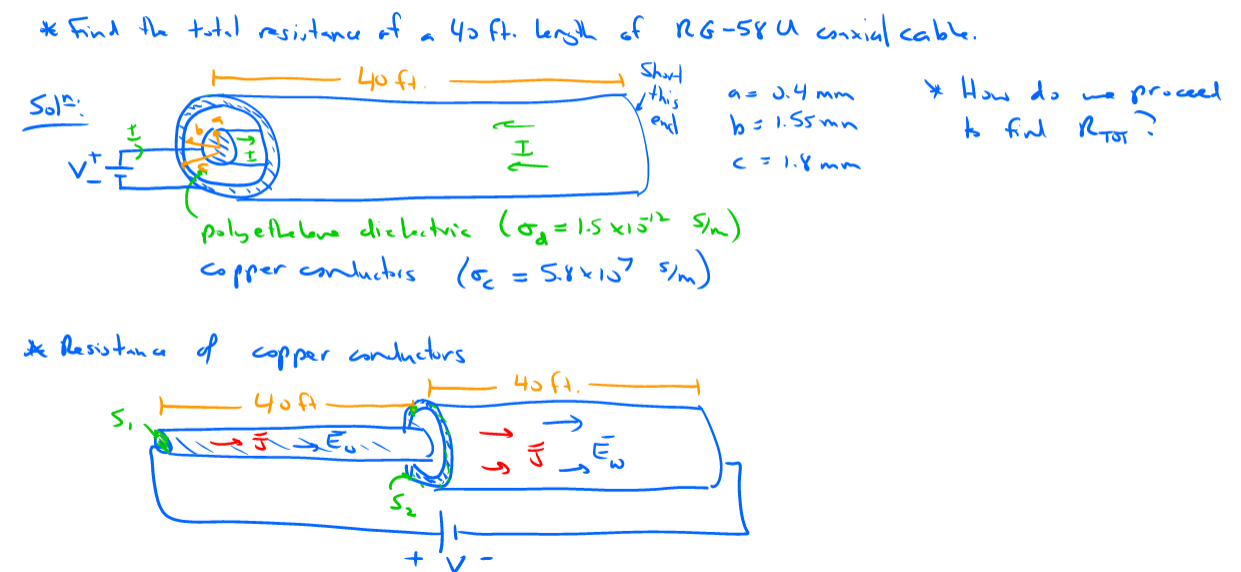
\includegraphics[width=0.7\textwidth]{coaxial.png}
	\end{figure}
	\begin{align*}
		R &= \frac{L_1}{\sigma S_1} + \frac{L_2}{\sigma S_2} \\
		  &= \frac{40\times0.305}{5.8\times10^7\pi a^2} + \frac{40\times0.305}{5.8\times10^7\pi(c^2-b^2)} \\
		  &= 485\unit{m\Omega}
	\end{align*}
	Using Guass' Law,
	$$\vec{E} = \frac{\rho_{sa}a}{\varepsilon_0\varepsilon_r}\hat{a}_r$$
	So
	$$R = \frac{\int_a^b \frac{\rho_{sa}a}{\varepsilon_0\varepsilon_r}dr}{\int_0^{2\pi}\int_0^L \frac{\sigma_d \rho_{sa}a}{\varepsilon_0\varepsilon_r a} adzd\phi} = \frac{\ln\frac{b}{a}}{2\pi L\sigma_d} = 1.17\times10^{10} \unit{\Omega}$$
	Alternatively,
	$$R = \int\frac{dl}{\sigma_d S} = \int_a^b \frac{dr}{\sigma_d \times 2\pi rL} = \frac{\ln\frac{b}{a}}{2\pi L\sigma_d}$$
	giving the same result.
\end{ex}

\section{Joule's Law}

Joule's Law addresses power loss, as electric field has to do work to create a current.

\begin{align*}
	\Delta P &= \frac{d\Delta U}{dt} \\
		 &= \frac{d}{dt} \int\vec{F}_e \cdot d\vec{l} \\
		 &= \frac{d}{dt}\int Q\vec{E} \cdot d\vec{l} \\
		 &= \frac{d}{dt} \int\rho_v \Delta V \vec{E} \cdot d\vec{l} \\
		 &= \int \vec{E} \cdot \left(\rho_v \frac{d\vec{l}}{dt}\right) \Delta V \\
		 &= \vec{E} \cdot \vec{J} \Delta V
\end{align*}
Where we substitute the definition of $\vec{J}$ on the last equality.

\end{document}
